%Preamble
\documentclass[12pt,a4paper]{article}        %Define text type and basic formatting
%\usepackage[document]{ragged2e}   %Text alignment https://www.overleaf.com/learn/latex/Text_alignment

\usepackage[utf8]{inputenc}     %Usage of UTF-8 for umlauts
\usepackage[ngerman]{babel}     %Paper language;
\pagenumbering{arabic}  % "Normal" page numbering
%Set line spacing to 1.5
% \usepackage{setspace}
% \onehalfspacing

%Citation and reference
\usepackage[backend=biber,
  style=authoryear,
  citestyle=authoryear-comp,
  hyperref=true,
  giveninits,    %Shorten first names to initial
  uniquename=init,    %prevent name disambiguation
  sorting=nyt,  % sort by name, year, title
  natbib,  %enable citep/citet(parentheses only around year)
  maxbibnames=99,  %show all names in bibliography (no influence on in-text citation)
  minbibnames=1  %show at least one name before et al
]{biblatex}   %REFERENCES https://www.overleaf.com/learn/latex/Bibliography_management_in_LaTeX
\addbibresource{references.bib}     %Lib file
\usepackage[nottoc,numbib]{tocbibind}   %add bibliography to toc

%page citation in text with colon: https://tex.stackexchange.com/questions/433122/changing-comma-in-textcite-to-colon
%\DeclareFieldFormat{postnote}{#1}
%\DeclareFieldFormat{multipostnote}{#1}
%\renewcommand\postnotedelim{\addcolon\addspace}

% Ensure "S." appears before page numbers in citations
\DeclareFieldFormat{postnote}{S.~#1}
\DeclareFieldFormat{multipostnote}{S.~#1}

% Handle comma between author and year and et al.
\renewcommand\nameyeardelim{\addcomma\space} %comma between author and year
%u.a. as et al.
\DefineBibliographyStrings{german}{%
  andothers = {et al.},
}
%Replace and/und with &
\renewcommand*{\finalnamedelim}{%
  \ifnumgreater{\value{liststop}}{2}{\finalandcomma}{}%
\addspace\&\space}%

% Easier inline citation -> \say{} command
\usepackage{dirtytalk} 

%images
\usepackage{graphicx}       %Required for adding images
\graphicspath{{images/}}    %image path
\usepackage{wallpaper}  %Page background img

\usepackage{parskip}        %Prevent indention of paragraphs
\usepackage{mathtools}    %required for math formulas
\usepackage{amssymb}    %mathematical symbols
\usepackage{listings}   %For code listings

%Use markdown in LaTex https://de.overleaf.com/learn/latex/Articles/How_to_write_in_Markdown_on_Overleaf
\usepackage[footnotes,definitionLists,hashEnumerators,smartEllipses,hybrid]{markdown}

\usepackage{titlesec}   %Style titles
\usepackage{fancyhdr}   %Header/footer
%\usepackage[bottom]{footmisc}   %Foot notes, at end of page

%Links
\usepackage[colorlinks,
  pdfpagelabels,
  pdfstartview = FitH,
  bookmarksopen = true,
  bookmarksnumbered = true,
  linkcolor = black,
  plainpages = false,
  hypertexnames = false,
  citecolor = black,
urlcolor = black]{hyperref}   %Hyperref pkg -> clickable links and TOC
\usepackage{csquotes}   % Autostyle quotes language-specific

%Font settings
\renewcommand{\familydefault}{\sfdefault}       %Text sans-serif
\renewcommand{\headrulewidth}{0pt}
\pagestyle{fancy}

%Footer
\fancyhf{}      %Clear all header/footer stylings
% \lfoot{\thedate\hspace{1pt}}
% \cfoot{Proposal Bachelorarbeit\\«Video- und bildbasierte Desinformation auf Social-Media-Plattformen in der Schweiz» (Arbeitstitel)} % Footnote
\rfoot{\thepage\hspace{1pt}}        %Add page number

%Title page settings
\usepackage{pdfpages}
\usepackage{titling}    %Title page styling
\title{«Analyse (audio-) visueller Desinformation auf Social-Media-Plattformen in der Schweiz» (Arbeitstitel)}        %Document Title
\author{Yannick Spriessler}     %Author of paper
\date{\today}     %Date of paper; ALTERNATIVE: \today

% Separate bibliography for images
% \defbibheading{imagecredits}{\section*{Bildverweis}}
% \addbibresource{img-references.bib}

%___________________________________________________________________________________________
%TITLE PAGE
\begin{document}
\begin{titlingpage} %Start titling page
  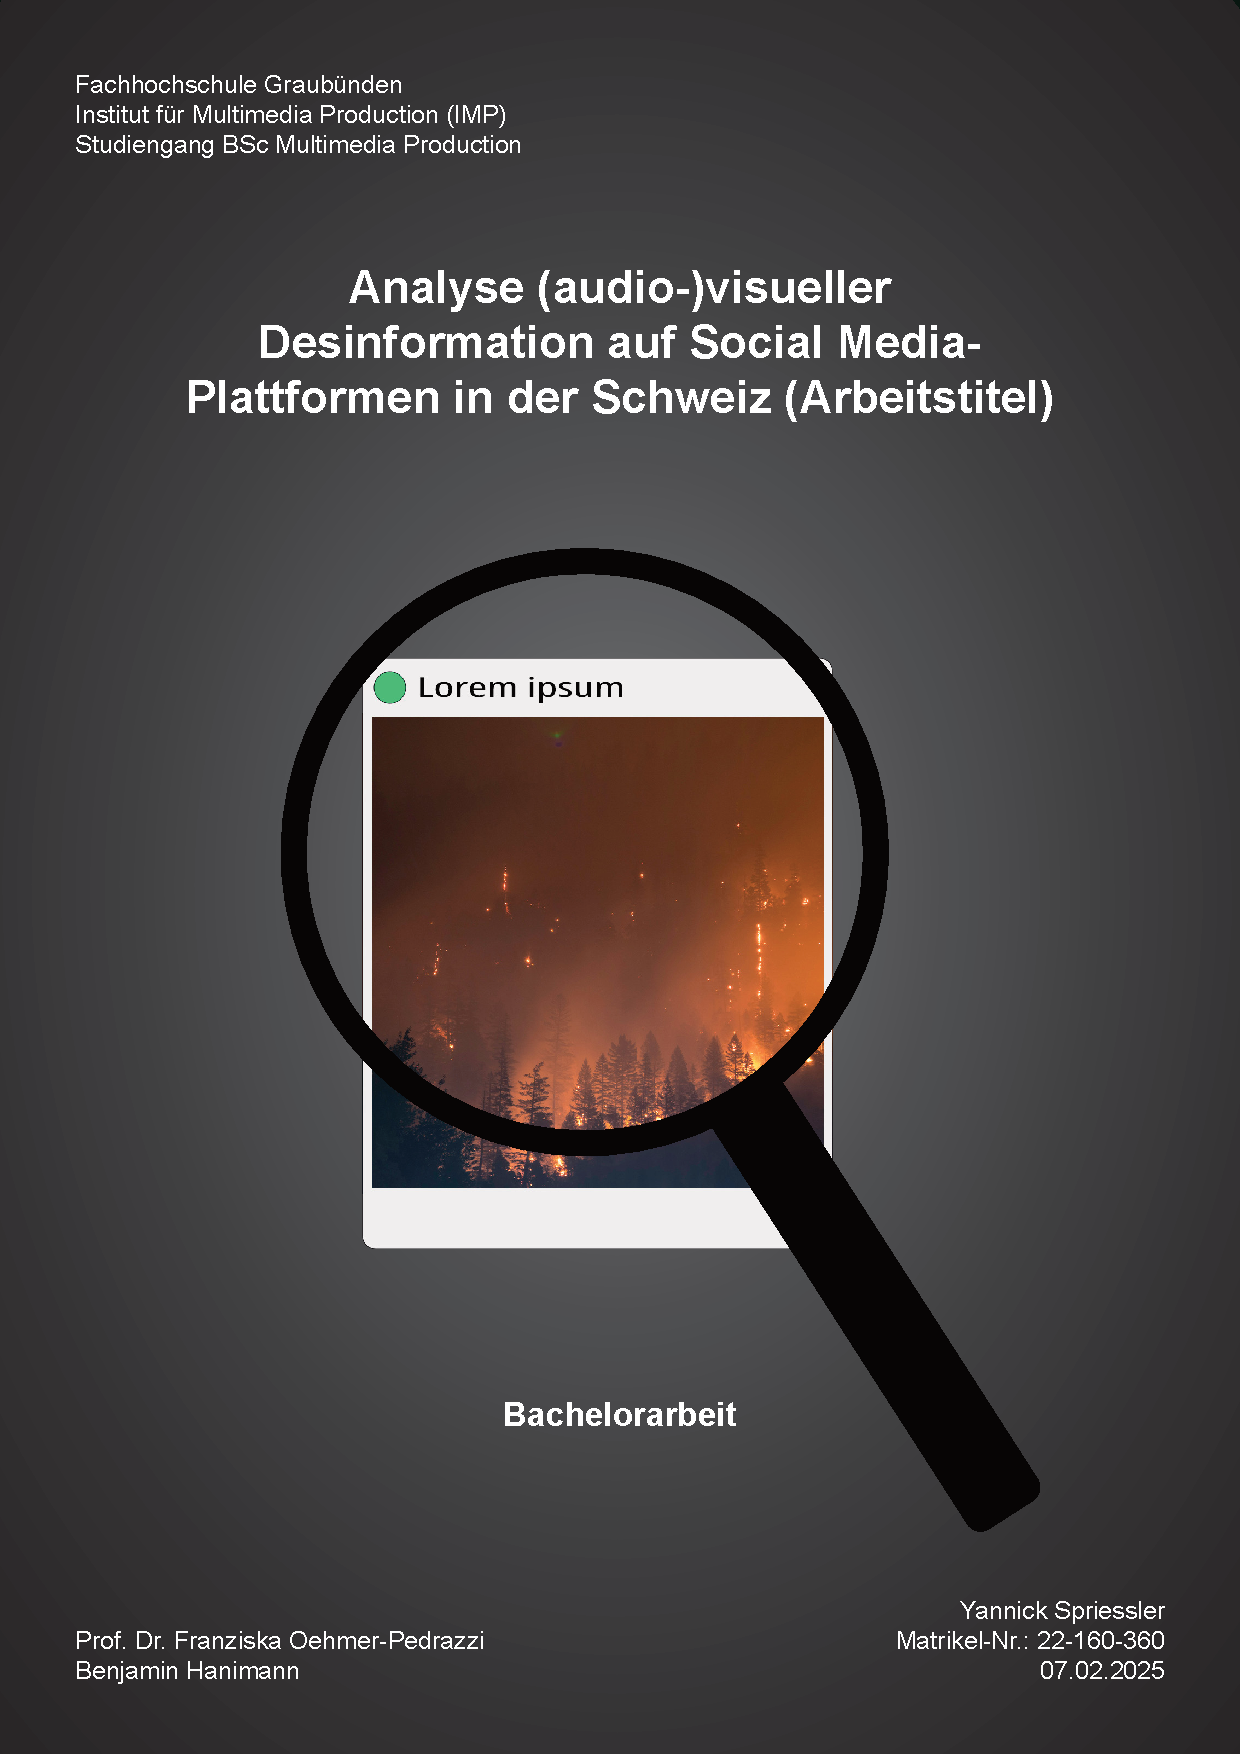
\includepdf{Titelblatt_Thesis}
  \nocite{howard_trees_2017}  %Citation for title page, only in image bibliography
\end{titlingpage}
\pagebreak      %Insert page break
%-----------------------------------------------
\renewcommand{\abstractname}{Abstract}
\begin{abstract}
  \setlength{\parindent}{0pt}  
    asdfghjk \\
\end{abstract}

\textbf{Keywords:} \textit{Desinformation, Social Media, audiovisuelle Inhaltsanalyse}


\textbf{Zitiervorschlag:}
\linebreak
%\frontmatter   %If foreword
\pagebreak
%TOC
\thispagestyle{empty}
\setcounter{page}{0}    %Set page no.
\tableofcontents        %Content index
\pagebreak
%-----------------------------------------------
%DOC

%\mainmatter    %Main part if foreword used
\section{Einleitung}
Spätestens seit den US-Wahlen 2016 hat der Begriff «Fake News» stark an Bedeutung gewonnen. Zwar handelt es sich dabei nicht um eine Neuerscheinung und falsche Informationen wurden lange vor der Entwicklung des Internets verbreitet \parencites[214]{allcott_social_2017}[247]{hohlfeld_schlechte_2020}[1]{khan_fake_2021}, dennoch ist das Problem unter anderem durch die Verbreitung über das Internet weiter stark angewachsen \parencites[214–215]{allcott_social_2017}[1]{khan_fake_2021}[1]{lazer_science_2018}[4]{ceron_fake_2021}. \\
Aufgrund der sozialen Medien und der Möglichkeit, innerhalb kürzester Zeit Videos und Bilder zu produzieren, können heute sehr schnell audiovisuelle Falschinformationen verbreitet werden. Diese stellen nicht nur ein Problem für die individuellen Rezipierenden dar, sondern gefährden dabei auch politische und gesellschaftliche Prozesse.

Die Bachelorarbeit befasst sich damit, welche inhaltlichen und gestalterischen Merkmale audiovisuelle und bildbasierte Desinformation auf Social-Media-Plattformen in der Schweiz aufweist. \\
Ziel der Arbeit ist es zum einen herauszufinden, ob es mögliche Muster und
Strategien hinter der Produktion der Inhalte gibt. Zum anderen soll auch ein
allgemeines Verständnis über die entsprechenden Inhalte gewonnen werden. \\
Die Erkenntnisse der Bachelorarbeit werden anschliessend verwendet, um darauf basierend eine interaktive Aufklärungsplattform zu gestalten.

\subsection{Relevanz}
\textbf{Gesellschaft}
\linebreak
Im Jahr 2024 betrug der Anteil der Social-Media-Nutzenden in der Schweiz knapp 80 \%. Weiter informiert sich ein bedeutender Anteil der europäischen Bevölkerung über das Internet, eine Mehrheit verwendet Social Media primär für Nachrichten und Unterhaltung \parencite[21ff]{we_are_social_anteil_2024}. Gemäss der JAMES-Studie 2024 \parencite[40]{kulling-knecht_james_2024} informiert sich 2024 etwa die Hälfte der Jugendlichen täglich oder mehrmals pro Woche auf sozialen Plattformen. \\
Somit wird durch Social-Media-Inhalte ein Grossteil der Schweizer Bevölkerung erreicht. Dadurch können desinformierende Inhalte potenziell einen grossen Einfluss auf die Bevölkerung und ihre (politische) Meinungsbildung haben \parencites[18]{grujic_warnhinweise_2024}[258]{hohlfeld_schlechte_2020}[1f]{khan_fake_2021}, insbesondere wenn Social-Media-Plattformen auch als Informationsquelle zu politischen und gesellschaftlichen Themen dienen.

\textcite{grady_neural_1998} haben gezeigt, dass sich Rezipierende besser und länger an visuelle Inhalte erinnern können als an Worte. Eine weitere Untersuchung fand einen Zusammenhang zwischen dem Konsum von Videos und der Möglichkeit der Nutzenden, auf diese zu reagieren \parencite[242]{khan_social_2017}. Inhalte mit Partizipationsmöglichkeit scheinen ausserdem den weiteren Konsum (information seeking) zu befeuern \parencite[243]{khan_social_2017}. \\
Insofern kann davon ausgegangen werden, dass audiovisuelle Desinformation eine besondere Gefahr darstellt. 

\textbf{Politik}
\linebreak
\textcite[258]{hohlfeld_schlechte_2020} schreiben Desinformation die Fähigkeit zu, demokratische Gesellschaften \say{durch Inhalte, die Angst und Verunsicherung schüren, [\ldots] [sowie, d. Verf.] durch die Schwächung der seriösen Institutionen der Erkenntnisbeschaffung und [\ldots] durch Normverschiebungen des politisch Sagbaren} zu destabilisieren. \parencite[vgl.\ auch][1]{khan_fake_2021}.

Eine Marketingfirma fand 2016 heraus, dass Fake-News-Seiten für die Verbreitung ihrer Inhalte fast komplett abhängig von Facebook sind. Während solche Seiten 50 \% der Websitebesuche von Facebook erhalten, lagen seriöse Medien bei etwa 20 \%.\parencites{wong_almost_2016}[zit.\ nach][1]{khan_fake_2021}[vgl.\ auch][212]{allcott_social_2017}. \\
Facebook und weitere Social-Media-Plattformen können somit als starke Treiber von Desinformation verstanden werden \parencite{wong_almost_2016}. In Anbetracht der jüngsten Tendenz, Einordnungen durch Faktencheck-Organisationen auf den Meta-Plattformen einzustellen \parencites{isaac_meta_2025}{meta_transparency_centre_penalties_2025}, ist es für die Nutzenden deshalb umso wichtiger, Inhalte bezüglich ihres Wahrheitsgehalts korrekt einordnen zu können. 

Gemäss dem \textcites{bundesministerium_des_innern_und_fur_heimat_desinformation_2022}\parencite[zit.\ nach][15]{teetz_social-media-post_2023} kann Desinformation in einigen Fällen sogar als Bedrohung der nationalen Sicherheit verstanden werden. \\
Die Schweiz hat mit ihrer direkten Demokratie ein weltweit einzigartiges politisches System, in keinem anderen Staat hat die Bevölkerung so viele Mitbestimmungsrechte \parencite[2]{sager_politische_2017}. Es ist deshalb zwingend notwendig, dass diese ihre politischen Entscheide aufgrund von korrekten Fakten und eigener politischer Entscheidung treffen kann, ohne von Desinformation beeinflusst zu werden \parencite[26]{vogler_wahrnehmung_2021}\parencite[vgl.\ auch][14f]{european_parliament_directorate-general_for_external_policies_of_the_union_impact_2021}. Auch wenn über die tatsächliche Gefährdung der Schweizer Politik durch Desinformation bisher noch wenig bekannt ist, scheint die Schweiz als Staat vergleichsweise widerstandsfähig zu sein (ebd.).\\
Durch das Wissen der Plattform-Nutzenden über Desinformation und die Mechanismen der Social-Media-Plattformen und die Fähigkeit, falsche von echten Tatsachen zu unterscheiden, kann diese Gefahr weiter verringert werden.

\textbf{Wissenschaft}
\linebreak
Soziale Medien funktionieren fundamental anders als traditionelle Medien. Nachrichten und andere Inhalte können ohne faktische Einordnung oder inhaltlichen Kodex weltweit geteilt werden \parencite[211]{allcott_social_2017}. Die journalistischen Kriterien wie \say{Unabhängigkeit,  Ausgewogenheit, Vielfalt, Verständlichkeit und Unterhaltsamkeit}\parencite[9]{grujic_warnhinweise_2024} werden nicht überprüft. Besonders in Krisenzeiten sind die Nutzenden besonders anfällig für Falschinformationen \parencite[vgl.][2]{ceron_fake_2021}. \\
Social-Media-Plattformen und ihre entsprechenden Algorithmen zur Inhaltsauswahl basieren neben den Interaktionen der Nutzenden untereinander in ihrer Funktionsweise vor allem auf der Generierung von Aufmerksamkeit \parencites[vgl.][220]{schmidt_meinungsbildung_2022}[493]{behnke_manipulation_2018}. \\
Durch die Verbreitung eines Inhaltes wird zwangsläufig die Kapazität der Nutzenden für die Verarbeitung anderer Inhalte geschmälert \parencite[248]{hohlfeld_schlechte_2020}.

Die Wissenschaft kennt das Potenzial und die Gefahr von Social-Media-Plattformen, durch Fragmentierung und das Anzeigen bestimmter Inhalte Filterblasen zu schaffen und die Gesellschaft zu spalten – dieser Effekt konnte jedoch bisher nicht tatsächlich bewiesen werden \parencite[220]{schmidt_meinungsbildung_2022}.

Als Massnahme gegen Desinformation werden oft Faktenchecks eingesetzt. Deren Wirksamkeit wird allerdings immer wieder in Frage gestellt \parencites[1095]{lazer_science_2018}[4f]{ceron_fake_2021}. \say{(\ldots) people prefer information that confirms their preexisting attitudes (selective exposure), view information consistent with their preexisting beliefs as more persuasive than dissonant information (confirmation bias), and are inclined to accept information that pleases them (desirability bias).} \parencites[1095]{lazer_science_2018}\parencite[vgl.\ auch][18]{grujic_warnhinweise_2024}. Faktenchecks könnten in einigen Fällen sogar kontraproduktiv sein, wenn  die Falschinformation wieder aufgefrischt wird und dadurch eher hängenbleibt als die faktische Einordnung (ebd.). Umso wichtiger ist es, dass die Rezipierenden die medialen Artefakte möglichst selbst beurteilen können.

\subsection{Forschungsfrage}
Folgende Fragestellung wird in der Bachelorarbeit behandelt:

\begin{quote}
  Welche inhaltlichen und gestalterischen Merkmale weist visuelle und audiovisuelle Desinformation auf Social-Media-Plattformen in der Schweiz auf?
\end{quote}
\color{red}Begründung für Forschungsfrage.


\color{red}Aufbau der Arbeit 
\color{black}
\pagebreak
\section{Forschungsstand}

\textbf{Begriffsdefinition}

Beispielsweise durch die Präsidentschaft des US-Präsidenten Donald Trump (2017–2021) oder den Brexit hat der Begriff «Fake News» weltweit an Bedeutung gewonnen \parencites[1f]{hohlfeld_schlechte_2020}[1]{marx_fake_2020}. \\
In der Literatur existieren verschiedene Definitionen des Begriffes. \textcite[246f]{hohlfeld_schlechte_2020} vertreten beispielsweise die Haltung, dass «Fake News» als Begriff für desinformierende Inhalte gleichbedeutend sind mit dem politischen Propagandabegriff. In den letzten Jahren wurde allerdings auch oft argumentiert, dass «Fake News» lediglich als politischer Begriff gewertet und im wissenschaftlichen Kontext stattdessen von (aktueller) Desinformation gesprochen werden sollte \parencites[3]{bontridder_role_2021}{habgood-coote_stop_2019}[148]{marx_fake_2020}. Egelhofer \& Lecheler \parencite[zit.\ nach][148]{marx_fake_2020} differenzieren zwischen «Fake News» als Genre für Falschinformationen und «Fake News» als Label im Sinn einer politischen Instrumentalisierung zur Diskreditierung von Medien und Institutionen.\\
In Anlehnung an \textcite{marx_fake_2020} und in Abgrenzung zum politischen Label wird in dieser Bachelorarbeit der Begriff «Desinformation» verwendet.

In der Wissenschaft gibt es bisher keine einstimmige Definition für Desinformation. 
\textcite[148f]{marx_fake_2020} benennen ein Theoriendefizit, basierend auf widersprüchlichen Definitionen sowie nicht-nachvollziehbaren Definitionskriterien.\\
Laut \textcite[1094]{lazer_science_2018} handelt es sich bei Desinformation um \say{fabricated information that mimics news media content in form but not in organizational process or intent. Fake-news outlets, in turn, lack the news media’s editorial norms and processes for ensuring the accuracy and credibility of information.}
\textcite[213]{allcott_social_2017} sprechen von \say{(\ldots) news articles that are intentionally and verifiably false, and could mislead readers.} \parencites[vgl.\ auch][140]{tandoc_defining_2018}[1094]{lazer_science_2018}.\\
Diese Definition kann nicht nur auf News-Artikel angewendet werden, sondern auch auf andere mediale Artefakte \parencite[3]{bontridder_role_2021}. \textcite[1]{marx_fake_2020} definieren aktuelle Desinformation als \say{Kommunikation wissentlich und empirisch falscher Informationen zu neuen und relevanten Sachverhalten mit dem Anspruch auf Wahrheit.} Sie stützen sich dabei auf folgende Kriterien:

\begin{itemize}
  \item \textbf{(Visuelle) Kommunikation}: Eine wahrheitsfähige Mitteilung mit repräsentationalem Gehalt, welche einen Wirklichkeitsausschnitt abbildet. Dies bezieht sich nicht nur auf sprachliche, sondern auch auf visuelle Mitteilungen \parencite[151]{marx_fake_2020}.
  \item \textbf{Aktualitätsbezug}: \say{(\ldots) überraschende Themen mit (potenziell) großer Auswirkung auf die Gesellschaft. So ermöglicht sie ihrem Publikum die Ausbildung von (wenn auch empirisch unzutreffenden [\ldots]) Erwartungen und dadurch die Orientierung in einer komplexen Welt.} \parencite[152]{marx_fake_2020}.
  \item \textbf{Wahrheitsanspruch}: Aktuelle Desinformation beansprucht für sich, dass sie (vorgetäuscht) wahr ist. In diese Betrachtung werden sowohl Produzierende wie auch Rezipierende des Inhaltes miteinbezogen. Hierbei gilt, ob es für externe Beobachtende plausibel ist, dass Rezipierende die Nachricht als wahr betrachten \parencite[153]{marx_fake_2020}.
  \item \textbf{Unwahrheit}: Der desinformierende Inhalt besitzt irreführendes Potenzial, da er empirisch falsch ist und somit den zuvor beanspruchten Wahrheitsgehalt nicht einlöst. \parencite[154]{marx_fake_2020}.
  \item \textbf{Unwahrhaftigkeit}: Die Produzierenden sind sich der Tatsache bewusst, dass ihre Mitteilungen falsch sind. \parencite[156]{marx_fake_2020}
  \item \textbf{Täuschungsabsicht}: Falsche Tatsachen werden vorsätzlich und bewusst verbreitet. Dabei spielt es keine Rolle, ob diese der gezielten Verbreitung von Falschinformationen dienen sollen oder beispielsweise zu Clickbait-Zwecken eingesetzt werden \parencites[157]{marx_fake_2020}[vgl.\ auch][2]{khan_fake_2021}. 
\end{itemize}

Desinformation muss abgegrenzt werden von weiteren verwandten Themen und Begriffen:

\begin{itemize}
  \item \textbf{Missinformation}: Missinformation \say{ (\ldots) refers to false, inaccurate, or misleading information that is shared without any intent to deceive.} \parencite[2]{bontridder_role_2021}. \citeauthor{marx_fake_2020} grenzen Missinformation anhand des Unwahrhaftigkeitskriteriums ab, indem es sich bei Missinformation gemäss ihrer Definition um eine unwissentliche Fehlinformation handelt \parencite[156]{marx_fake_2020}, welche ohne Täuschungsabsicht verbreitet wird \parencite[vgl.\ auch][15]{grujic_warnhinweise_2024}.
  \item \textbf{Satire}: Satire ist nach \textcite[154]{marx_fake_2020} erkennbar an einer klaren Quelle (beispielsweise ein Satiremagazin) sowie bestimmten Text- und Stilmerkmalen und grenzt sich von Desinformation ab durch den Verzicht auf den Wahrheitsanspruch. Diese Einschätzung wird ebenfalls durch externe Beobachtende getroffen.\\
  Weitere Merkmale sind humoristische oder übertriebene Darstellungen \parencites[141]{tandoc_defining_2018}[2]{khan_fake_2021}, obwohl diese auch in seriösen und korrekten Nachrichten verwendet werden können.
  \item \textbf{Gerücht}: Ein Gerücht zeichnet sich dadurch aus, dass sein Wahrheitsgehalt (noch) nicht überprüft ist \parencite[155]{marx_fake_2020}. Der Wahrheitsgehalt von Desinformation lässt sich jederzeit prüfen.
  \item \textbf{Verschwörungstheorie}: Rosnow \& Kimmel \parencite[zit.\ nach][197]{krafft_disinformation_2020} definieren Verschwörungstheorien (Rumors) als \say{an unverified proposition for belief that bears topical relevance for persons actively involved in its dissemination.} (ebd.). \textcite[197]{krafft_disinformation_2020} halten eine persönliche Betroffenheit sowie Informationsunsicherheit als Bedingungen für eine Verschwörungstheorie fest.\\
  Von Desinformation unterscheidet sich eine Verschwörungstheorie dadurch, dass sie meist auch von denjenigen geglaubt wird, welche zu ihrer Verbreitung beitragen \parencite[156]{marx_fake_2020}.
  \item \textbf{Fake News}: Zum einen wird der Begriff im politischen Kontext als abwertendes Label verwendet für Nachrichten, welche nicht nach dem Gusto der politischen Akteurinnen und Akteure berichten \parencite[3]{tandoc_jr_facts_2019}.\\
  Zum anderen handelt es sich bei «Fake News» um eine Unterkategorie der Desinformation, welche spezifisch Nachrichtenartikel bezeichnet, welche Falschinformationen beinhalten und so aufbereitet sind, dass sie für echt gehalten werden (können) (ebd.).
\end{itemize}

\citeauthor{marx_fake_2020} haben in ihrer Arbeit eine Begriffsdefiniton für aktuelle Desinformation aufgestellt, welche den Term klar definiert und von anderen Kategorien von Falschinformationen abgrenzt. In dieser Bachelorarbeit wird nachfolgend ihre Definition zur Beurteilung von Desinformation angesetzt.

\subsection{Aktuelle Desinformation}
Wie in vielen Publikationen festgehalten
Desinformation kein neues Phänomen; Verbreitung heute vor allem online, u.a. durch fehlende Regulation
- Wo treffen wir auf Desinformation? \\
- Auswirkungen\\
- Wer verbreitet Desinformation?\\
- Wie wird Desinformation verbreitet?\\
- Motivation hinter der Verbreitung von Desinformation\\
- Zu welchen Themen?\\
- (Erkennungsmerkmale)

\pagebreak
\section{Methode}
\subsection{Methodenwahl}
\subsection{Untersuchungszeitraum}
\subsection{Räumlicher Geltungsbereich}
\subsection{Analysegegenstand}
\subsubsection{Methodisches Vorgehen}
\subsubsection{Auswertung}
\pagebreak
\section{Ergebnisse}
\pagebreak
\section{Schlussteil}
\subsection{Diskussion}
\subsection{Beantwortung der Forschungsfrage}
\subsection{Weiterer Forschungsbedarf}

\pagebreak
%-----------------------------------------------
%BIB
\section{Verzeichnisse}
\subsection{Literatur}
\printbibliography[heading=none, nottype=artwork]
 \subsection{Bildverweise}
 \printbibliography[heading=none, type=artwork] %Only reference artworks
 \subsection{Abbildungsverzeichnis}
 \listoffigures[heading=none]
\subsection{Hilfsmittelverzeichnis}

\section{Anhang}
\end{document}
